\documentclass[11pt]{article}
\usepackage[utf8]{inputenc}	% Para caracteres en español
\usepackage{amsmath,amsthm,amsfonts,amssymb,amscd}
\usepackage{multirow,booktabs}
\usepackage[table]{xcolor}
\usepackage{fullpage}
\usepackage{algorithm}
\usepackage{algpseudocode}
\usepackage{lastpage}
\usepackage{enumitem}
\usepackage{listings}
\usepackage{fancyhdr}
\usepackage{mathrsfs}
\usepackage{wrapfig}
\usepackage{setspace}
\usepackage{calc}
\usepackage{multicol}
\usepackage{cancel}
\usepackage[retainorgcmds]{IEEEtrantools}
\usepackage[margin=3cm]{geometry}
\usepackage{amsmath}
\newlength{\tabcont}
\setlength{\parindent}{0.0in}
\setlength{\parskip}{0.05in}
\usepackage{empheq}
\usepackage{framed}
\usepackage[most]{tcolorbox}
\usepackage{xcolor}
\colorlet{shadecolor}{orange!15}
\parindent 0in
\parskip 12pt
\geometry{margin=1in, headsep=0.25in}
\theoremstyle{definition}
\newtheorem{defn}{Definition}
\newtheorem{reg}{Rule}
\newtheorem{exer}{Exercise}
\newtheorem{note}{Note}
\begin{document}
\title{Operating System}
\author{fl\_334}
\date{}
\thispagestyle{empty}
\maketitle

\tableofcontents
\clearpage
\section{Intro to OS}
    \subsection{Computer System Components}
    \begin{itemize}
        \item \textbf{Hardware}
        \begin{itemize}
            \item Basic Computing Resources(CPU, memory...)
        \end{itemize}

        \item \textbf{Operating Systems}
        \begin{itemize}
            \item Control and Coordination: Manage hardware usage for diverse user applications.
        \end{itemize}

        \item \textbf{Application Programs}
        \begin{itemize}
            \item Resource Utilization: Utilize system resources to solve problems or complete tasks.
        \end{itemize}

        \item \textbf{Users}
        \begin{itemize}
            \item User Types: People, machines, or other computers interacting with the computer system.
        \end{itemize}
    \end{itemize}
\subsection{Functions of Operating Systems}
    \begin{itemize}
        \item \textbf{Interface Between User and Hardware}
        \begin{itemize}
            \item Mediating User-Hardware Interaction
        \end{itemize}

        \item \textbf{Control Interactions Between Users and Programs}
        \begin{itemize}
            \item Managing User-Program Interactions
        \end{itemize}

        \item \textbf{Provides a Controlled and Efficient Environment}
        \begin{itemize}
            \item Efficiency and Control
        \end{itemize}

        \item \textbf{Provides Mechanisms and Policies}
        \begin{itemize}
            \item Resource Management
        \end{itemize}
    \end{itemize}
\subsection{OS History}
   \subsubsection{The First Computers}
        \begin{itemize}
            \item Early machines (1940s to mid-1950s) had no Operating System.
            \item The user interacted directly with the hardware.
            \begin{itemize}
                \item Initial interfaces: console of switches (input) \& lights (output).
                \item Later interfaces: punched cards, printers, etc.
            \end{itemize}
            \clearpage
            \item \textbf{Issues}
            \begin{itemize}
                \item Long setup time for a program to run.
                \item Users accessed the system one at a time.
                \item Scheduling made by hand.
                \item No sharing of libraries, drivers, and other resources.
            \end{itemize}
        \end{itemize}
    \subsubsection{Mainframes: Batch Systems}
    \begin{itemize}
        \item The earliest Operating Systems were used in mainframes (1950s).
        \item These OSs were batch systems, which aimed to eliminate the manual setup of programs to be run and provided reusable code to access hardware (i.e., drivers). The Operating System was stored in main memory (referred to as a monitor).
        \item One job (program) was loaded at a time from a punched card/tape reader into the remaining memory, and job control instructions told the Operating System what to do.
        \item These simple OSs were code to which one linked one's program (loaded as a whole into main memory) to be run, essentially functioning as a run-time library.
        \item \textbf{Issues}
            \begin{itemize}
                \item Input/output (I/O) operations were very slow.
                \item No computations were done while performing I/O.
                \item This decreased CPU usage.
            \end{itemize}
    \end{itemize}
    \subsubsection{Mainframes: Multiprogramming}
    \begin{itemize}
        \item Idea: Expand memory to hold two or more programs and switch among all of them (multitasking or multiprogramming).
        \item Multiprogramming systems became possible with the advent of the first integrated circuits (IC) in the early 1960s, aiming to increase processor utilization and optimize throughput (i.e., jobs completed per unit of time).
        \item The degree of multiprogramming refers to the number of jobs that can be managed at once by the OS.
        \item Multiprogramming (aka multitasking) is the central theme of modern OSs, where multiple runnable jobs are loaded in memory simultaneously, allowing overlap of I/O operations of one job with the computations of another.
        \item This approach benefits from I/O devices that can operate asynchronously, such as interrupts and direct memory access (DMA).
    \end{itemize}
    \newpage
    \subsubsection{Mainframes: Timesharing}
    \begin{itemize}
        \item Initially, multiprogramming was still batch-based:
        \begin{itemize}
            \item Turnaround time could be long for any particular job.
            \item No interactivity.
        \end{itemize}
        \item The idea was to have multiple users simultaneously using terminals, with the OS interleaving the execution of each user program in short quanta of computation.
        \item \textbf{Timesharing Systems}
        \begin{itemize}
            \item Based on time slicing (a.k.a. time multiplexing), where each user feels like using the shared computer as if it were their own.
            \item The challenge was to optimize response time.
            \item Timesharing systems allow users to view, edit, debug, and run their programs interactively.
    \end{itemize}
    \end{itemize}
   \subsubsection{Desktop Operating Systems (1980s)}
    \begin{itemize}
        \item Very Large Scale of Integration (VLSI) circuits made it cheaper to manufacture complex hardware.
        \item Hardware became cheaper.
        \item Easier to have one computer per user than share a mainframe.
        \item Usability was facilitated by the introduction of graphical user interfaces (GUI).
        \item The idea was to maximize user convenience and responsiveness, focusing on the user experience, apart from CPU and I/O considerations, similar to multiprogrammed and timesharing systems.
    \end{itemize}
    \subsubsection{Parallel Operating Systems}
    
    The concept behind Parallel Operating Systems is to efficiently run and manage parallel applications on tightly coupled parallel computers (multiprocessors). These operating systems provide support for parallel applications composed of several time-consuming but separable subtasks.

    Key features of Parallel Operating Systems include:

    \begin{itemize}
        \item Providing primitives for assigning (scheduling) parallel subtasks to different processors.
        \item Offering primitives for dividing a task into parallel subtasks, if possible.
        \item Supporting efficient communication between parallel activities.
        \item Enabling synchronization of activities to coordinate data sharing.
    \end{itemize}
    \subsubsection{Distributed Operating System}
    
    The concept behind Distributed Operating Systems is to have a common operating system shared by a network of loosely coupled independent computers. These systems facilitate the sharing of resources located in different places, both hardware and software, and appear to their users like an ordinary centralized operating system. Key features include:

    \begin{itemize}
        \item Supporting communication between parts of a job or between different jobs across the network.
        \item Allowing for some level of parallelism, although speed is not the primary goal.
    \end{itemize}

\subsubsection{Real-Time Operating System}
    
    Real-Time Operating Systems are designed to guarantee a response to physical events within a fixed interval of time. They are commonly used for specialized applications such as subway systems, flight control, factories, and power stations. Key characteristics of real-time operating systems include:

    \begin{itemize}
        \item Scheduling all activities to meet critical requirements and performing operations within predetermined timeframes.
        \item The distinction between "Hard real-time" for critical systems and "Soft real-time" implemented by all modern PC operating systems to run multimedia applications.
    \end{itemize}
\section{OS Structure}
    \subsection{OS System Components}
        \subsubsection{Process Manager}
            \begin{itemize}
                \item Process: Program in execution
                \item How to run and terminate a process
                \item Suspend/pause and resume a process
                \item Process synchronisation
                \item Inter-process communication
                \item Handling deadlocks
                \item Keep track what is running in the system
                \item Run the processes efficiently
            \end{itemize}
        \subsubsection{Main-Memory Management}
            \begin{itemize}
                \item Track what part of memory is being used and by which process
                \item Decide where to lead a process in the system
                \item Allocate and free memory as per required
            \end{itemize}
        \subsubsection{File Management}
            \begin{itemize}
                \item Create and delete files and directories
                \item Basic file and directory manipulation like read/write etc.
                \item Mapping the files into secondary storage, like a hard disk
            \end{itemize}
        \subsubsection{I/O System Management}
            \begin{itemize}
                \item A device driver interface
                \item Drivers for specific hardware
                \item A memory management component implementing buffering, caching and spooling
            \end{itemize}
        \subsubsection{Secondary-Storage Management}
            \begin{itemize}
                \item Free space management
                \item Storage allocation
                \item Disk scheduling
            \end{itemize}
        \subsubsection{Networking}
            \begin{itemize}
                \item Implement network stack
                \item Provide services to connect the OS to the network
            \end{itemize}
        \subsubsection{Protection System}
            \begin{itemize}
                \item Memory protection
                \item Device protection
                \item Memory protection...
            \end{itemize}
        \subsubsection{Command-Interpreter System}
            \begin{itemize}
                \item Provide an interface to the user so that they can use the services of the OS
                \item Can be a command line shell
                \item Can be a GUI
            \end{itemize}
        \subsubsection{Kernel}
            Software containing the core OS components; it may typically include:
            \begin{itemize}
                \item Memory Manager
                    \\ - Provides efficient memory allocation and deallocation of memory
                \item I/O Manager
                    \\ - Handles input and output requests from and to hardware devices(through device drivers)
                \item Inter-process communication (IPC) manager
                    \\ - Provides communication between different processes(programs in execution)
                \item Process Manager (scheduler)
                    \\ -Handles what is executed when and where (if more than one CPU)
            \end{itemize}
            A OS kernel may consist of many more components
            \begin{itemize}
                \item System service routines
                \item File System (FS) manager
                \item Error handling systems
                \item Accounting systems
                \item System programs
                \item And many more
            \end{itemize}
    \clearpage
    \subsection{Operating System Interface}
        - Original OS interfaces were very simple and called \textbf{Command Line Interface(CLI)} or \textbf{Command Interpreter(CI)}
        - The user types a command and the CI executes it
        - Later systems used a more user friendly Graphical User Interface(GUI)
        - Based on Desktop idea
            \begin{itemize}
                \item Usually mouse, keyboard, and monitor
                \item WIMP(windows, icons, menus, pointing)
                \item Icons represent files, programs, actions, etc
            \end{itemize}
        - Used on almost all systems today
        \begin{figure}
            \centering
            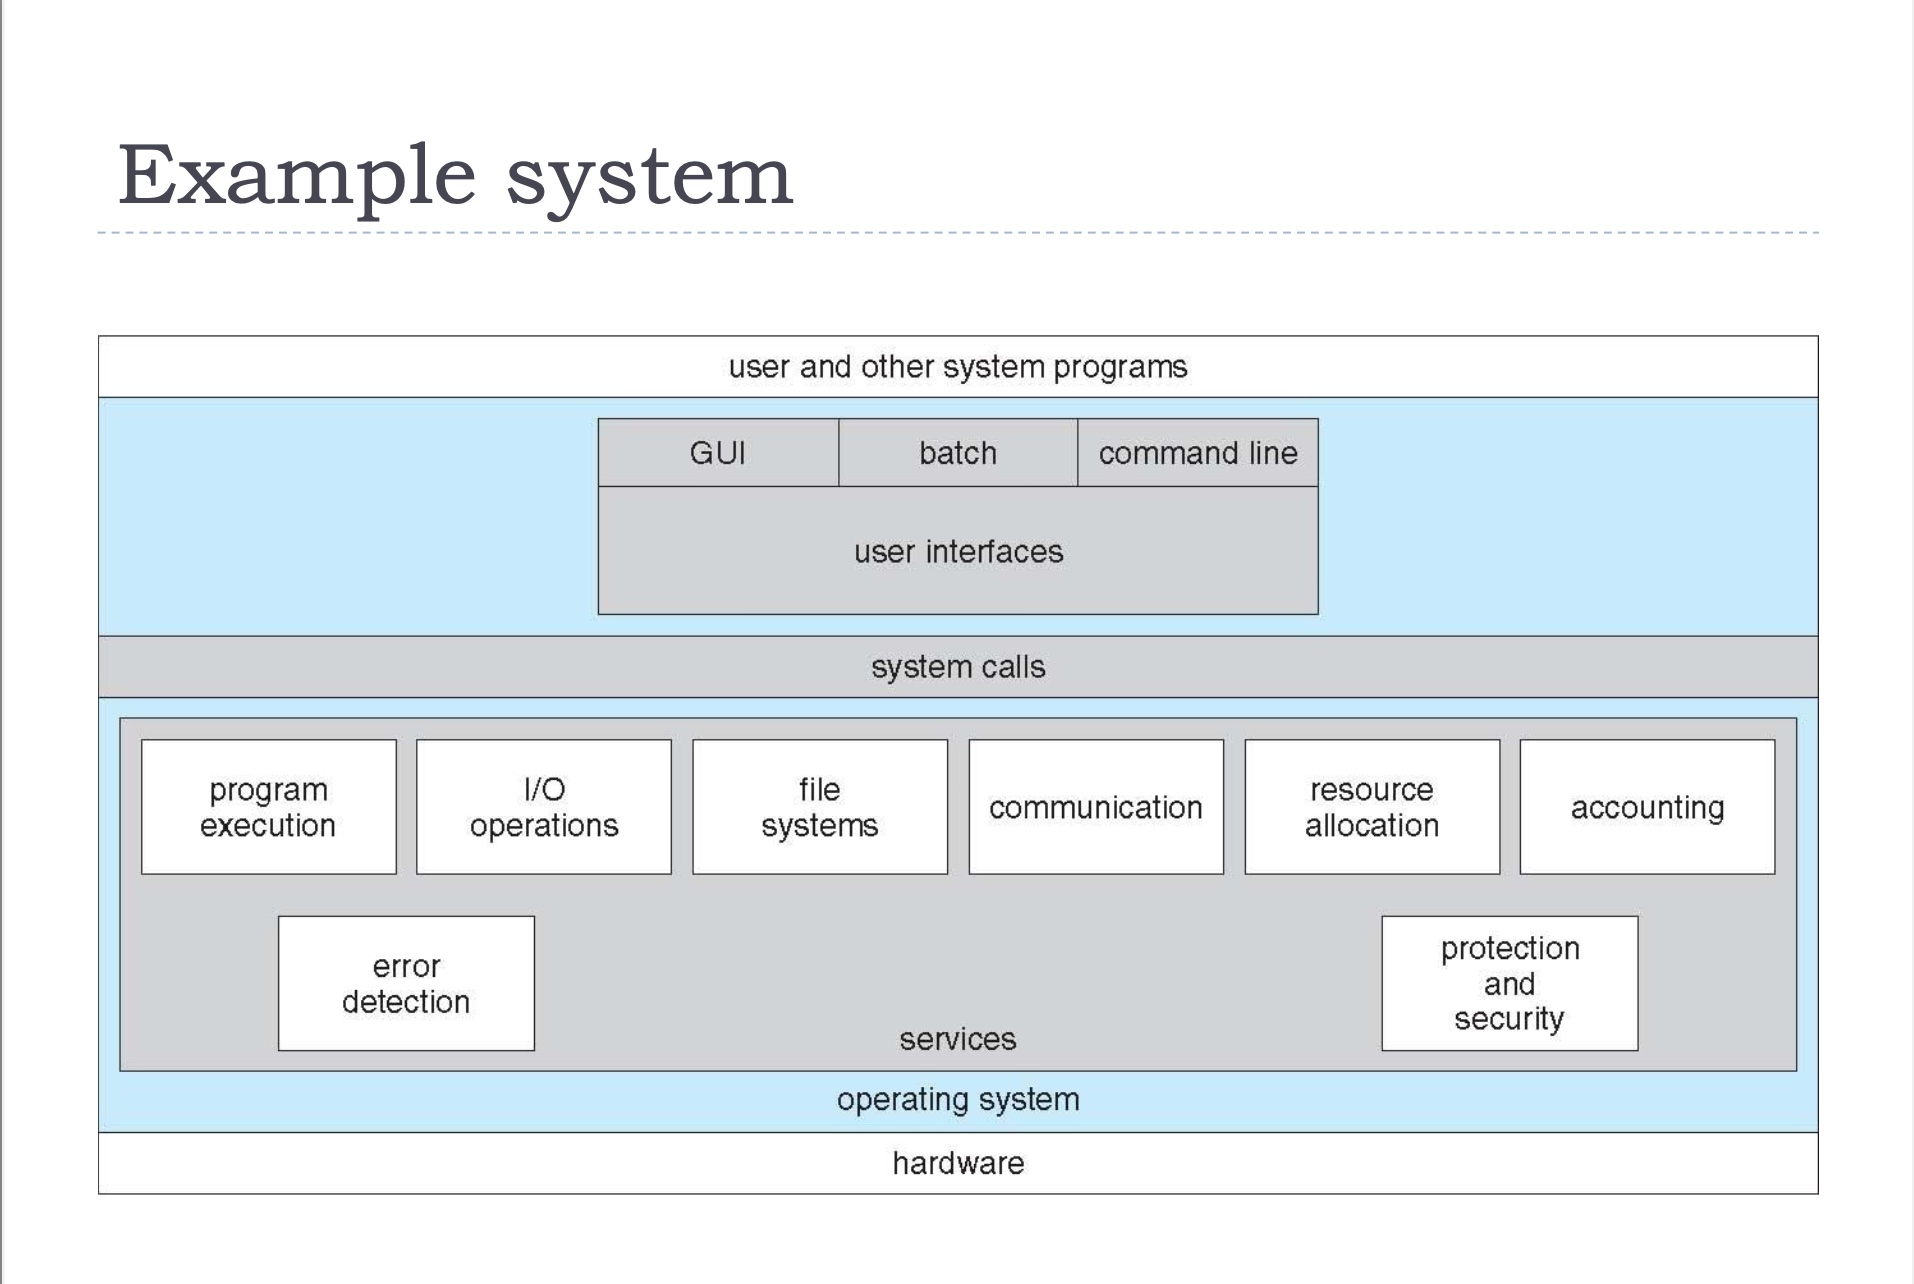
\includegraphics[width=1.0\linewidth]{img/Example_system.jpg}
            \label{fig:enter-label}
        \end{figure}
    \subsection{Monolithic Architecture}
        \begin{itemize}
            \item every OS component is contained in the kernel
            \item any component can directly communicate with any other(by means of function calls)
            \item due to this they tend to be highly efficient(performance)
            \item Example : MS DOS
                \begin{itemize}
                    \item Written to provide the most functionality in the least space
                    \item Not divided into modules
                    \item Interfaces and levels of functionality are not well separated
                \end{itemize}
            \item Problems
             \begin{enumerate}
                 \item Unstructured -- Hard to understand, modify and maintain
                 \item All kernel code runs with unrestricted access to the system \\-- Susceptible to damage from errant or malicious code 
             \end{enumerate}
        
             
        \end{itemize}

        \begin{figure}[h]
    \centering
    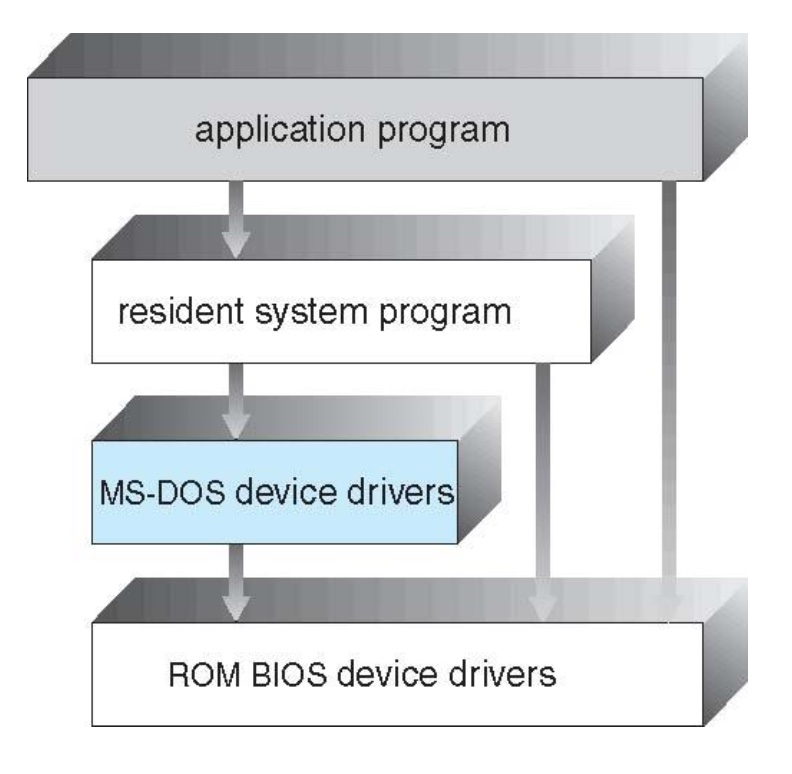
\includegraphics[width=0.4\textwidth]{img/MS_DOS.jpg} 
    \label{fig:a}
\end{figure}
    \subsection{Layered Structure}
        Component are grouped into layers that perform similar functions
        \subsubsection{First Layers-based OS}
            \begin{itemize}
                \item Layering was first used in Dijkstra's The OS(1968)
                \item Each layer "sees" a logical machine provided by the lower layers
                      \begin{itemize}
                            \item Layer 4(user space) sees virtual I/O devices
                            \item Layer 3 sees virtual console
                            \item Layer 2 sees virtual memory
                            \item Layer 1 sees virtual processors
                        \end{itemize}
                \item Based on a static set of cooperating systems
                \item Each process can be tested and verified independently
            \end{itemize}
        \subsubsection{Advantages}
            \begin{enumerate}
                \item Give the system structure and consistency for designing the system as a number of modules
                \item Allows easier debugging, modification and reuse
            \end{enumerate}
        \subsubsection{Layered Architecture}
            \hspace{1cm} Each layer communicates only with layers immediately above and below it
                \begin{itemize}
                    \item Each layer is a virtual machine to the layer above
                    \item A higher layer provides a higher-level virtual machine
                \end{itemize}
            \hspace{1cm} \begin{tabular}{|c|c|}
            \hline
                Layer 4 &  User Programs \\ \hline
                Layer 3 & I/O Management \\ \hline
                Layer 2 & Console Device(commands), IPC \\ \hline
                Layer 1 & Memory Management \\ \hline
                Layer 0 & CPU Scheduling (multiprogramming) \\ \hline
                        & Hardware \\ \hline
                
            \end{tabular}    
        \subsubsection{Problems}
            \begin{enumerate}
                \item Appropriate definition of layers is difficult
                    \begin{itemize}
                        \item A layer is implemented using only those operations provided by lower-level layers
                        \item A real system is often more complex than the strict hierarchy required by layering
                    \end{itemize}
                \item Not flexible
                    \begin{itemize}
                        \item The secondary memory(disk) driver woould normally placed \textbf{above} the CPU scheduler because an I/O wait may trigger CPU rescheduling operation
                        \item However, in a large system the CPU scheduler may need more memory than can fit in memory: parts of the memory can be swapped to disk(virtual memory), and then the secondary memory driver should be below the CPU scheduler
                    \end{itemize}
                \item Performance Issues
                    \begin{itemize}
                        \item Layer Crossing: Processes' requests might pass through many layers before completion
                        \item System throughout can be lower than in monolithic kernels
                    \end{itemize}
                \item Still susceptible to malicious/errant code
                    \begin{itemize}
                        \item If all layers have unrestricted access to the system
                        \item Can only be avoided through hardware
                    \end{itemize}
            \end{enumerate}
        \subsection{MircroKernel Architecture}
            \subsubsection{Architecture}
                \begin{itemize}
                    \item No agreement about minimal set of services inside the microkernel
                    \item At least: minimal process and memory mangament capabilities, plus inter-process communications
                    \item Services such as networking and file system tend to run nonprivileged at the user process level
                \end{itemize}
             \subsubsection{Benefits}
                \begin{itemize}
                    \item Modularity
                    \item Promote uniform interfaces
                    \item Distributed systems support \\
                        \hspace{1cm} Modules communicate through the microkernel, even through a network
                    \item Reliability
                    \item Scalability
                    \item Portability
                    \item Easy to extent and customise
                \end{itemize}
            \subsubsection{Disadvantages}
                System performance can be worse than in monolithic kernels, \\especially if kernel minimisation is taken too far
             \begin{figure}[htbp]
                \centering
                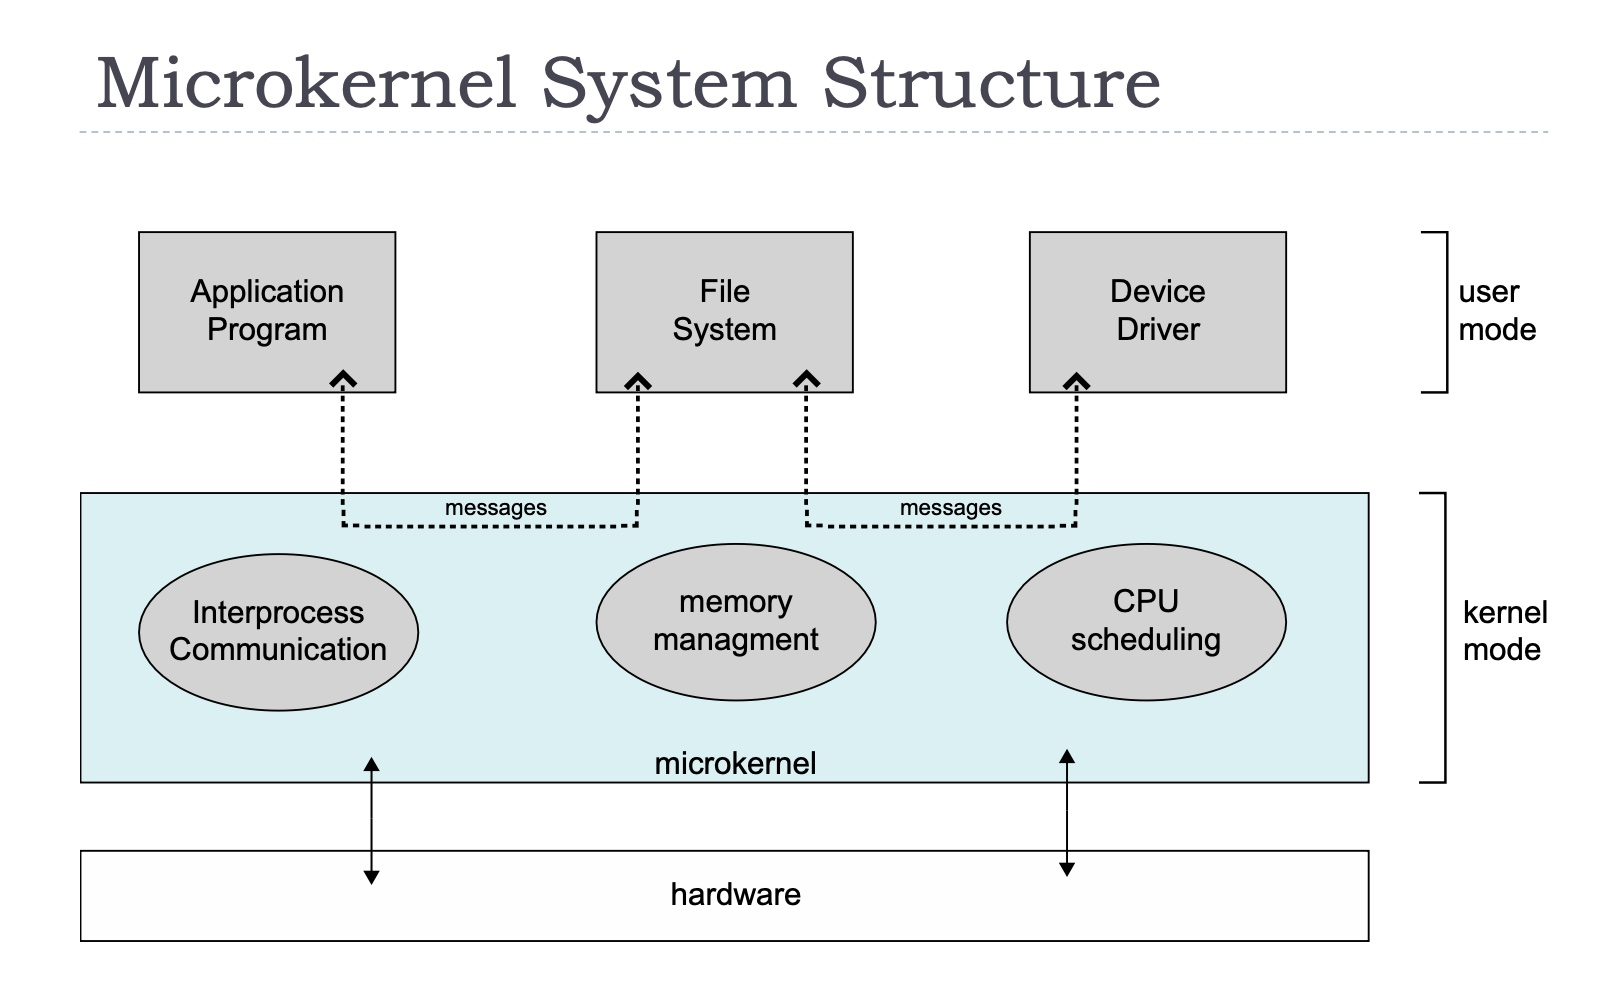
\includegraphics[width=0.65\linewidth]{img/microkernel.jpg}
                \label{fig:enter-label}
            \end{figure}
        \subsection{Modules}
        \hspace{1cm} Many modern operating systems implement loadable kernel modules
        \begin{enumerate}
            \item Uses object-oriented approach
            \item Each core component is separate
            \item Each talks to the others over known interfaces
            \item Each is loadable as needed within the kernel
        \end{enumerate}
        \hspace{1cm} Overall, similar to layers but with more flexibility (Linux, Solaris...)
        \begin{figure}[htbp]
                \centering
                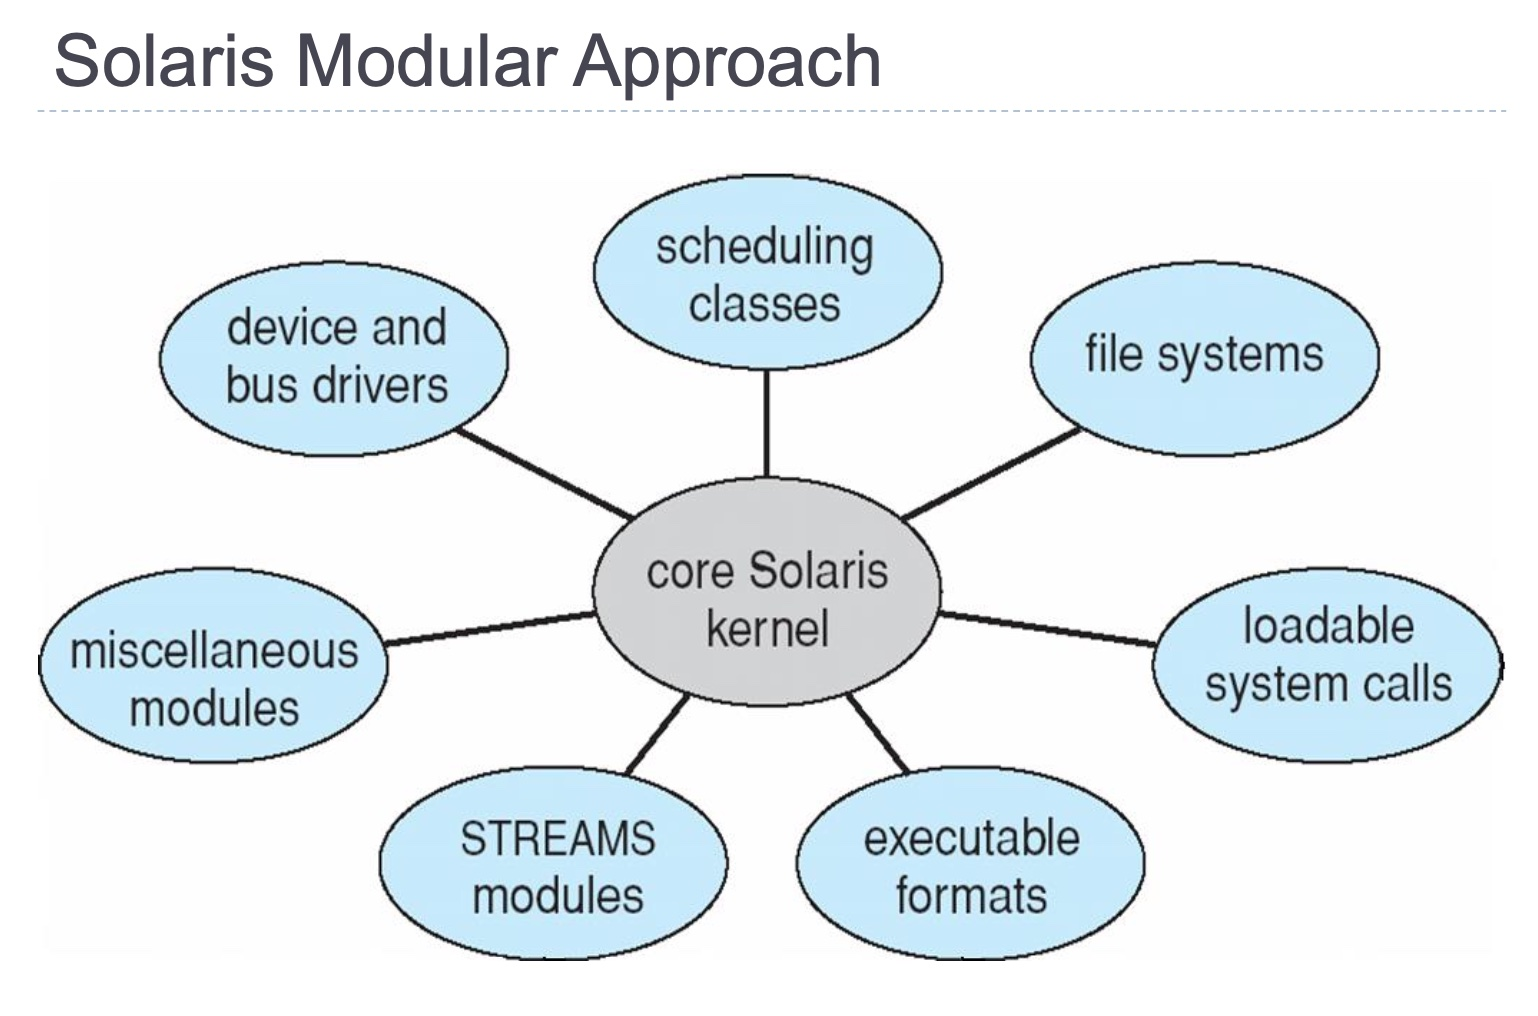
\includegraphics[width=0.65\linewidth]{img/Solaris_Modular_Approach.jpg}
                \label{fig:enter-label}
            \end{figure}
        \subsection{OS \& Hardware Features}
            \subsubsection{Protected Instructions}
                \begin{itemize}
                    \item Typically users are not allowed to
                    \begin{enumerate}
                        \item Directly access I/O (disk, printer, ...)
                        \item Directly manage memory
                        \item Execute CPU halt instructions
                    \end{enumerate}
                    \item These operations are always handled through privileged instructions or memory mapping
                \end{itemize}
            \clearpage
            \subsubsection{Dual Mode Operation}
                \begin{itemize}
                    \item The implementation of protected instructions required some type of hardware mechanism
                    \item The HW must support -at least two operation modes
                        \begin{itemize}
                            \item \textbf{kernel mode:} access to all the CPU instruction set // also called monitor/system/privileged mode
                            \item \textbf{user mode:} access restricted to a subset of the instruction set
                        \end{itemize}
                    \item The mode is indicated by a \textbf{status bit(mode bit)} in a protected processor register
                        \begin{itemize}
                            \item OS programs \& protected instruction executed in kernel mode
                            \item User programs executed in user mode
                        \end{itemize}
                    \item Examples of protection in older and newer systems
                        \begin{itemize}
                            \item \textbf{MS-DOS(based on Intel 8088):}no protection modes
                            \item \textbf{Windows 2000/XP, OS/2, Linux (based on Interl x86 systems):} protection modes
                        \end{itemize}
                \end{itemize}
            \subsubsection{Crossing Protection Boundries}
                \begin{itemize}
                    \item User-mode programs cannot execute privileged instructions but they still need kernel=mode services (I/O operations, memory management, etc)
                    \item To execute a privileged instruction, a user must call an OS procedure: \textbf{system call}
                    \item A system call causes a \textbf{trap}, which jumps to the trap handler in the kernel
                    \item When call the trap handler
                        \begin{itemize}
                            \item Uses call parameters to determine which system routine to run
                            \item Saves caller's state: Program counter(PC), mode bit, ...
                        \end{itemize}
                    \item After this the hardware mut
                        \begin{itemize}
                            \item Implement caller's parameters verification(e.g. memory pointers should only be allowed within user's section)
                            \item Return to user-mode when trap system call finished
                        \end{itemize}
                    \item The trap is treated by the hardware as a \textbf{software-initiated interrupt}
                \end{itemize}
                \clearpage
                \begin{figure}[t]
                \centering
                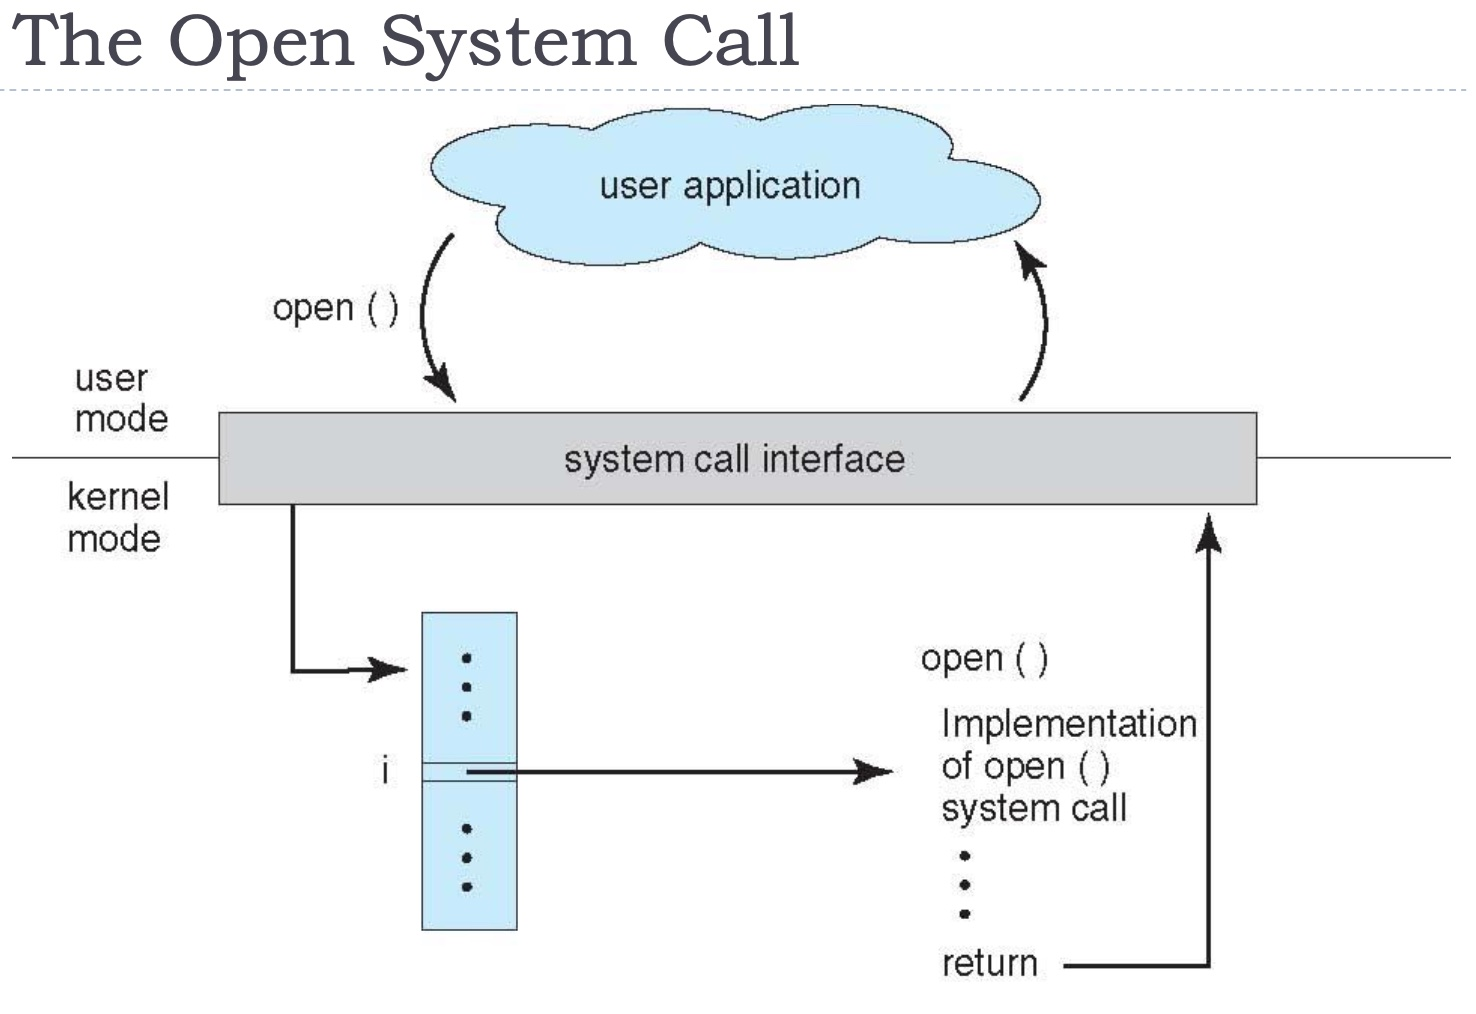
\includegraphics[width=0.6\linewidth]{img/open_system_call.jpg}
        
            \end{figure}
        \subsubsection{Exceptions}
            \begin{itemize}
                \item \textbf{Exception(hardware-initiated interrupt):} basically the same as a trap
                \item Automatically triggered by an error or a particular situation rather than on purpose(like in a system call)
                \item Transfer control to a handler within the OS \\ \hspace{1cm} System status can be saved on exceptions(memory dump) so faulty processes can be later debugged
                \item Decrease performance
                \\ \hspace{1cm} Exception conditions could be detected by inserting extra instructions in the code, but at a high performance cost
                \item Typical Exceptions
                    \begin{enumerate}
                        \item memory access out of user space
                        \item overflow, underflow
                        \item trace traps(debugging)
                        \item illegal use of privileged instructions
                        \item virtual memory(paging): page faults, write to read-only page
                    \end{enumerate}
            \end{itemize}
        \clearpage
        \subsubsection{Memory Protection}
            \begin{itemize}
                \item A memory protection mechanism must protect
                    \begin{itemize}
                        \item user programs from each other
                        \item OS(kernel) from user programs
                    \end{itemize}
                \item Simplest scheme is to use \textbf{base and limit registers}
                    \begin{itemize}
                        \item Based and limit registers are loaded by the OS before starting the execution of any program in user mode
                        \item base $\leq$ address $\le$ base + limit; otherwise exception raised
                    \end{itemize}
            \end{itemize}
        \subsubsection{I/O Control}
            \begin{itemize}
                \item All I/O instructions are privileged \\ \hspace{1cm} This is because a program could disrupt the whold system by issuing illegal I/O instructions
                \item Two situations must be considered:
                    \begin{itemize}
                        \item I/O start: handled by system calls
                        \item I/O completion and I/O events: handled by interrupts
                    \end{itemize}
                \item Interrupts are the basis for \textbf{asynchronous} I/O
                    \begin{itemize}
                        \item I/O devices have small processors that allow them to run autonomously (i.e. asynchronously with respect to the CPU)
                        \item I/O devices send interrupt signals when done with an operation; \\
                        CPU switches to address corresponding to interrupt
                        \\ an interrupt vector table contains the list of kernel routine addresses that handle different events
                    \end{itemize}
            \end{itemize}
        \subsubsection{CPU Protection}
            \begin{itemize}
                \item A user program might get stuck into an infinite loop and never return control to the OS
                \item \textbf{Timer:}it generates an interrupt after a fixed or variable amount of execution time
                \item When an interrupt is generated by the Timer the OS may choose to treat the interrupt as a fatal error and stop program execution or allocate more execution time
                \item In time-sharing systems a time interrupt is periodically generated after a fixed period of time for scheduling a new program
            \end{itemize}
            \clearpage
        \note{
            \begin{enumerate}
                \item An OS provides a number of services
                \item They relate to managing
                \begin{enumerate}
                    \item The hardware
                    \item The processes
                    \item The users
                    \item Communication between all of them
                \end{enumerate}
                \item Multiple ways of structuring the kernel, the system programs and user programs
                \item Each has advantags and disadvantages
            \end{enumerate}
            \hspace{1cm} \begin{tabular}{|c|c|}
            \hline
                OS Requirement &  Hardware Feature \\ \hline
                Dual kernel/user modes & Protected instructions \\ \hline
                System calls & Trap instructions and vectors \\ \hline
                Exceptions, signals & Interrupt vectors \\ \hline
                Memory protection & Base and limit registers \\ \hline
                I/O control        & Interrupts \\ \hline
                CPU protection, scheduling & Time (clock) \\ \hline
                
            \end{tabular}    
        }
    \clearpage
    \section{Processes \& Threads}
        \subsection{Processes}
        \subsubsection{Program}
        \begin{itemize}
            \item A program is a \textbf{passive} enitty stored on a disk
            \item A program becomes a process when it is \textbf{loaded into memory}
            \item One program can be many processes
        \end{itemize}
        \subsubsection{Process in memory}
        \begin{itemize}
            \item A process is a program in execution
            \item \textbf{text:} The program code
            \item Current activity including \textbf{program counter, processor registers}
            \item \textbf{Stack} containing temporary data
            \item \textbf{Data} section containing global variables
            \item \textbf{Heap} containing memory dynamically allocated during run time
        \end{itemize}
            \begin{figure}[htbp]
            \centering
                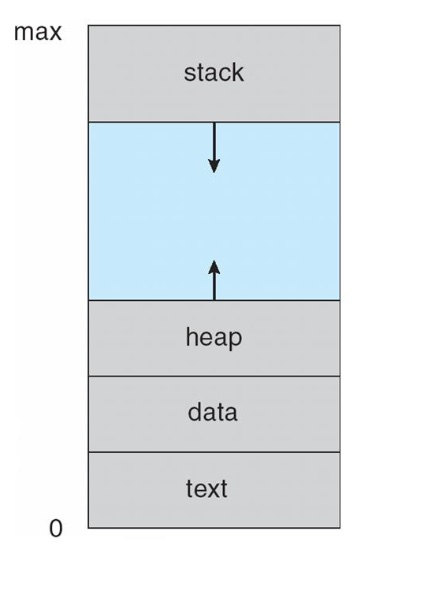
\includegraphics[width=0.30\linewidth]{img/process_in_memory.jpg}
                \label{fig:enter-label}
            \end{figure}
        \subsubsection{Process in Operating System}
        \begin{itemize}
            \item Each process runs in its \textbf{own address space}
            \item The \textbf{same} address in two different processes will be stored in two \textbf{different} locations in memory
        \end{itemize}
        \subsubsection{Process States}
            \begin{itemize}
                \item - \textbf{New:} The process is being created
                \item \textbf{Running:} Instructions a re being executed
                \item \textbf{Waiting:} The process is waiting for some event to occur
                \item \textbf{Ready:} The process is waiting to be assigned to a processor
                \item \textbf{Terminated:} The process has finished
            \end{itemize}
          \begin{figure}[htbp]
            \centering
                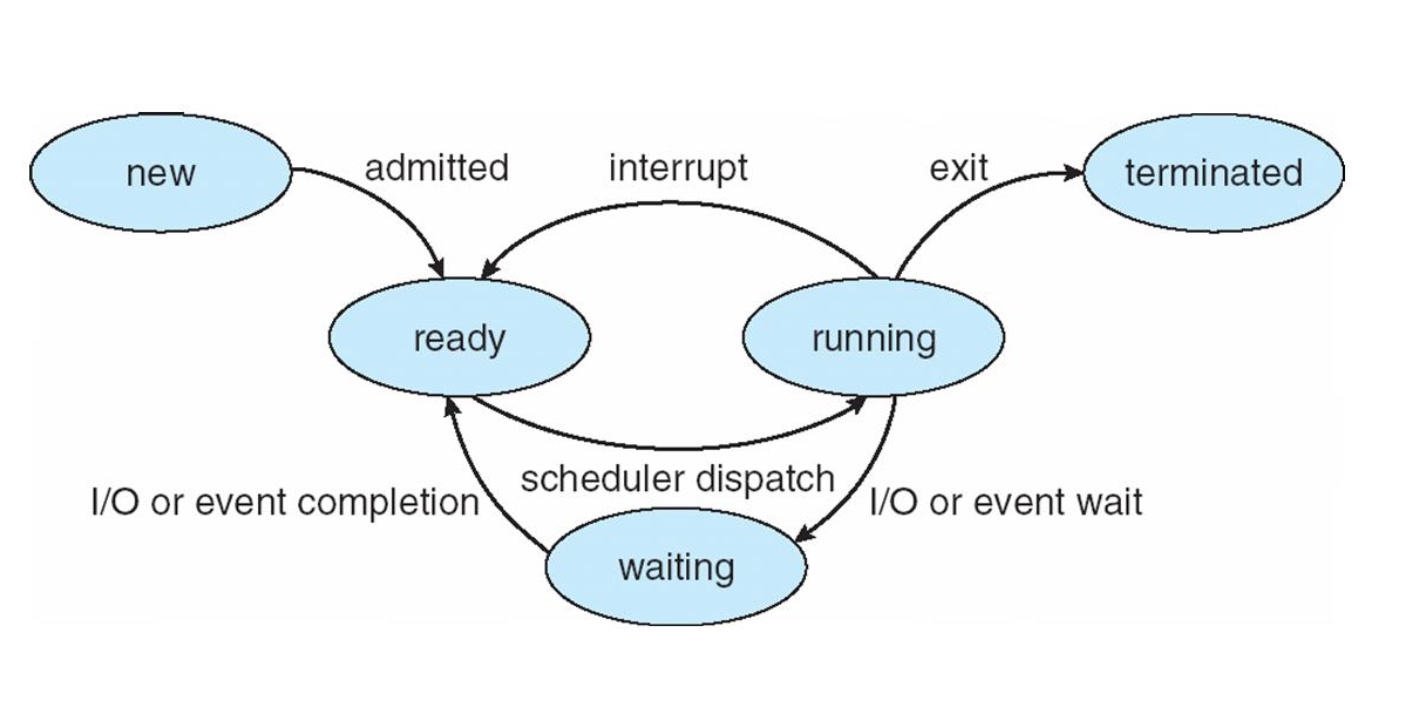
\includegraphics[width=0.80\linewidth]{img/process_states.jpg}
                \label{fig:enter-label}
            \end{figure}
        \subsubsection{Process Control Block(PCB)}
        \begin{itemize}
            \item PCB contains information associated with each process ( also called task control block)
            \item The OS keeps a either a system-wide or a per-user process table
            \item each entry contains a PID and a pointer giving the address of that process's PCB in memory
            \item Process state: running, waiting etc.
            \item Program Counter (PC): location of the next instruction to execute
            \item CPU registers - contents of all registers for this process
            \item CPU scheduling information - priorities, sheduling queue pointers
            \item Process number(PID)
            \item Memory-management information - memory allocated to the process
            \item Accounting information: CPU used, clock time elapsed since start, time limits
            \item I/O status information: I/O devices allocated to process, list of open files
        \end{itemize}
        \begin{figure}[htbp]
            \centering
                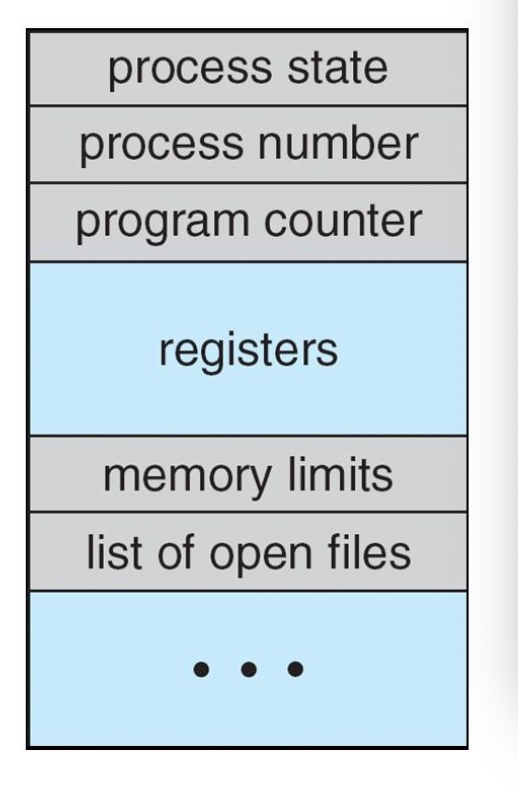
\includegraphics[width=0.30\linewidth]{img/PCB.jpg}
                \label{fig:enter-label}
            \end{figure}
        \subsubsection{Process Switching}
            \item Using the information stored in the PCB the OS can easily save and load the state of a process
            \item This allow processes to be easily switched; this is called a \textbf{context switch}
        \begin{figure}[htbp]
            \centering
                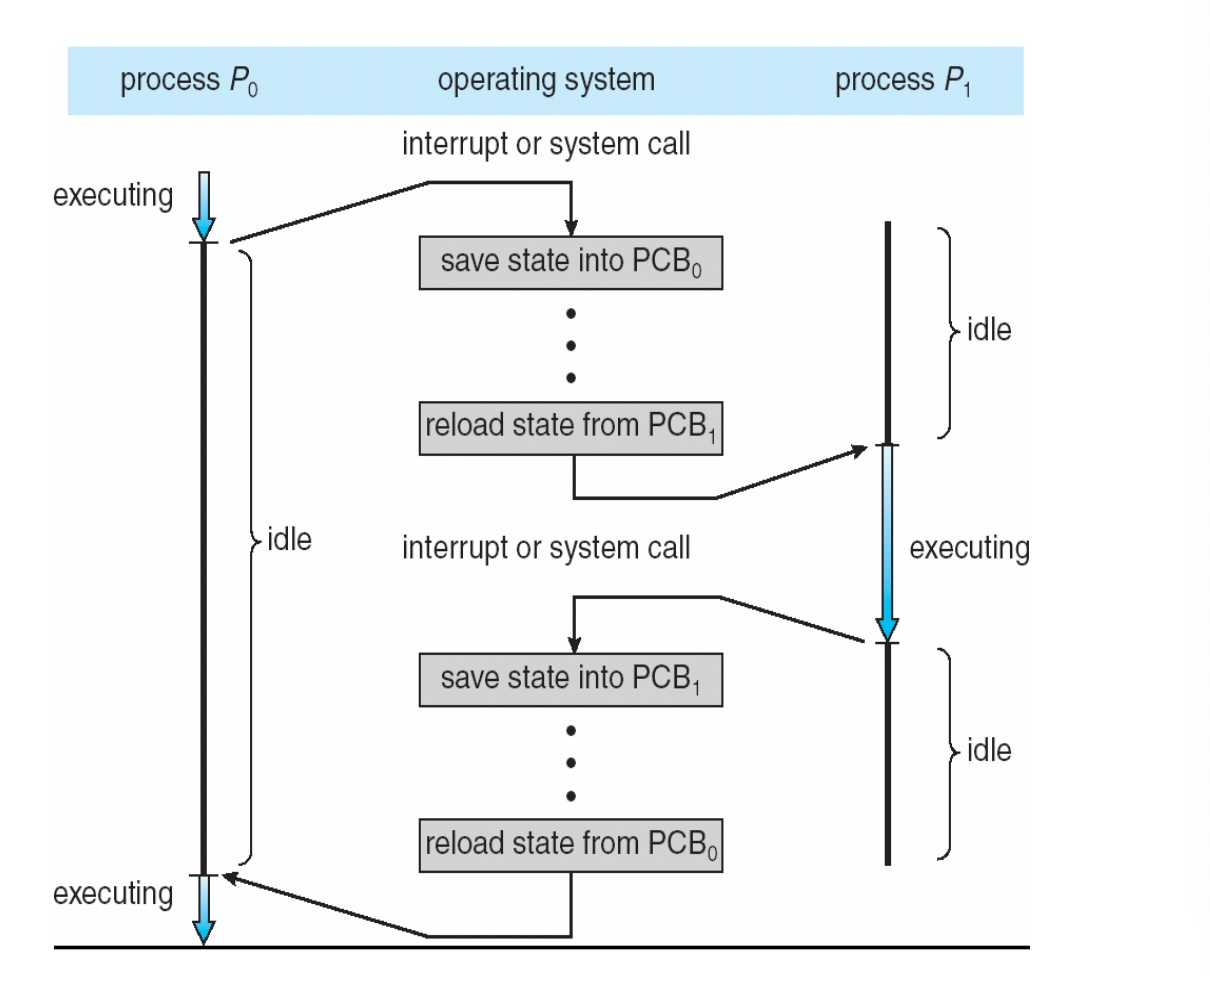
\includegraphics[width=0.68\linewidth]{img/Process_Switching.jpg}
                \label{fig:enter-label}
        \end{figure}
        \subsubsection{Overhead in Context Switch}
            \begin{itemize}
                \item While a context switch is happening, the system is not doing any work
                \item The time taken is considered the \textbf{overhead} of the operation
                \item To minimise the amount of time wasted context switches must be fast (hardware dependent)
                \item Also we don't want to switch too much(too much overhead) or too little(not interactive enough)
            \end{itemize}
        \subsubsection{Process Creation}
        Processes are created by two main events
        \begin{itemize}
            \item System boot
            \item Execution of process creation system call by another process
        \end{itemize}
        \subsubsection{Process Termination}
        Processes are terminated in different conditions:
        \begin{itemize}
            \item \textbf{Voluntary:} normal exit, error exit
            \item \textbf{Involuntary:} fatal error, killed by another process
        \end{itemize}
        voluntary termination can \textbf{only} happen from the running state\\
        Involuntary termination can happen from \textbf{any} state
        \subsubsection{Child Processes}
            \begin{itemize}
                \item \textbf{Process Tree:} A hierarchical process structure is created in this way(any child process only has one parent)
                \item An \textbf{orphan process} is a computer process whose parent has stopped but the process remains running
                \item Normally these processes are adopted by another parent process
                \item If this does not happen, they become a \textbf{zombie} process
                \item They should then be removed or reaped from the system
                \item A failure to reap a zombie process is normally due to a bug in the operating system
                \item Example(Unix)
                    \begin{itemize}
                        \item A child process is created using the fork() system call
                        \begin{itemize}
                            \item To the parent the fork system return the PID of the new child process
                            \item To the child it will return zero
                        \end{itemize}
                        \item The child receives almost everything from its parents
                        \item In essence the parent address \& PCB are copied
                        \item The child process must have a new PID, and will have different pointers for its parent/child processes
                        \item Because the PCB is copied the child process begins execution after the fork() instruction
                    \end{itemize}
            \end{itemize}
        \subsubsection{Interprocess Communication(IPC)}
            \begin{itemize}
                \item Independent Processes
                    \begin{itemize}
                        \item Those that can neither affect nor be affected by the rest of the system
                        \item Two independent processes cannot share system state or data
                        \item e.g.: processes running on different non-networked computers
                        \item \textbf{Deterministic} behaviour: only the input state determines the results and the results are \textbf{reproducible}
                        \item Can be stopped and restarted without any problems
                    \end{itemize}
                \item Cooperative Processes
                    \begin{itemize}
                        \item Share something
                        \item Two processes are cooperative if the execution of one of them may affect the execution of the other
                        \item e.g.: processes that share a single file system
                        \item \textbf{Nondeterministic} behaviour : many factors may determine the result and results may be difficult to reproduce
                        \item Make testing and debugging difficult
                        \item Subject to \textbf{race conditions}
                        \item Result may depend on the sequence or timing of events in other processes
                    \end{itemize}
            \end{itemize}
            \subsubsection{Issues}
                \begin{itemize}
                    \item Not efficient
                        \begin{itemize}
                            \item Creation of a new process is costly
                            \item all the process structures must be allocated upon creation
                        \end{itemize}
                    \item don't directly share memory
                        \begin{itemize}
                            \item Each process runs in its own address space
                            \item But parallel and concurrent processes often want to manipulate the same data
                            \item Most communications go through the OS: \textbf{slow}
                        \end{itemize}
                \end{itemize}
        \subsection{Thread}
            \begin{itemize}
                \item The idea is that there is more than one active entity(thread of control) within a single process
                \item Concurrency in some existing OS 
                \begin{itemize}
                    \item MS-DOS: one address space, one thread
                    \item Unix(originally): multiple address spaces, one thread per address space
                    \item OSX, Solaris, Windows 10: multiple address spaces, multiple threads per address space (multi-threading)
                \end{itemize}
                \item Threads \& Processes
                \begin{itemize}
                    \item  \textbf{Process:} defines the address space and general process attributes 
                    \item \textbf{Thread:} defines a single sequential execution stream within a process 
                    \item All threads belonging to a process share almost everthing in the process:
                    \begin{itemize}
                        \item Address space (code and data)
                        \item Global variables
                        \item Privileges
                        \item Open files
                        \item Timers
                        \item Signals
                        \item Semaphores
                        \item Accounting information
                    \end{itemize}
                    \item Threads however \textbf{do not share}
                    \begin{itemize}
                        \item Register set, in partucular
                        \begin{itemize}
                            \item Program counter(PC)
                            \item Stack pointer(SP)
                            \item Interrrupt vectors
                        \end{itemize}
                        \item Stack
                        \item State
                        \item Child threads
                    \end{itemize}
                    \item Cheap to create(no need to allocate PCB, new address space)
                    \item Communicate with each other efficiently through the process global variables or through common memory, using simple primitives
                    \item Facilitate concurrency, and therefore are useful even on uniprocessor systems
                    \item Threads can be created statically or dynamically (by a process or by another thread)
                    \item If a thread needs a service provided by the OS (system call) it acts on behalf of the process it belongs to
                    
                \end{itemize}
                \item Thread Implementations
                    \begin{itemize}
                        \item In user space(many-to-one model)
                        \begin{itemize}
                            \item The kernel schedules \textbf{processes} (does not implement or know about threads)
                            \item \textbf{per process thread table:} process decides which of its threads to run when it is running
                            \item Advantages
                            \begin{itemize}
                                \item A single-threaded OS can emulate multi-threading
                                \item thread scheduling controlled by run-time library, no system call overheads
                                \item portability: a OS independent user-space threads library is possible
                            \end{itemize}
                            \item Disadvantages
                            \begin{itemize}
                                \item If a thread blocks, all other threads belonging to the same process are blocked too
                                because the OS only schedules processes
                            \end{itemize}
                        \end{itemize}
                        \item In kernel space(kernel threads, one-to-one model)
                        \begin{itemize}
                            \item The kernel schedules threads
                            \item In this case threads are the smallest units of scheduling
                            \item \textbf{System-wide thread table} (similar to a process table)
                            \item Advantages
                            \begin{itemize}
                                \item Individual management of threads
                                \item Better interactivity
                            \end{itemize}
                            \item Disadvantages
                            \begin{itemize}
                                \item Scheduling and synchronisation operations always invoke the kernel, which increases overheads
                                \item Less portable
                            \end{itemize}
                        \end{itemize}
                        \item Hybrid(many-to-many model)
                    \end{itemize}
            \end{itemize}
    \section{Process Synchronisation}
    \subsection{Concurrent Execution}
        \begin{itemize}
            \item Concurrent Execution is when two processes are executing at the same time
            \item Each cooperative processes may affect the execution of the other process
                \begin{itemize}
                    \item by changing the resources available
                    \item by changing the value of memory
                \end{itemize}
        \end{itemize}
    \subsection{Atomic Operations}
        \note References and assignment are all \textbf{atomic} in the CPU

        
         All read and write operations happen as a single step.

         An atomic operation cannot be interrupted to prevent illogical things happening
    \subsection{Atomic Instructions}
    This atomicity is provided by hardware

    
    Higher-level constructs are not atomic in general


    A higher-level construct is any sequence of two or more instructions


    \note Process synchronisation is all about making high-level constructs behave atomically

    \subsection{Mutual Exclusion \& Critical Section}
    \subsubsection{Important Definitions}
    \begin{defn}[Synchronisation]
        Ensuring proper cooperation among processes or threads by relying on atomic operations
    \end{defn}
    \begin{defn}[Mutual Exclusion(ME)]
        ENsuring that only one process at a time holds or modifies a shared resource
    \end{defn}


    ME ensures atomicity
    \begin{defn} [Critical Section(CS)]
        A section of code in a program win which share resources are manipulated
    \end{defn}
    Mutual exclusion in a critical section requires serialisation of process access to the critical section
    \subsection{Locking and Mutual Exclusion}
        Achieving mutual exclusion in a critical section always involve some sort of \textbf{locking mechanism}


        Locking is where we prevent someone else for doing something with the shared resource


        Locking involves three rules:
        \begin{itemize}
            \item Lock before entering a critical section
            \item Unlock when leaving a critical section
            \item Wait when trying to enter critical section if it is locked
        \end{itemize}
        \clearpage
        \subsubsection{Requirements for True Solution for CS}
        \begin{itemize}
            \item Mutual exclusion
            \begin{enumerate}
                \item One process at most inside the CS at any time
            \end{enumerate}
            \item Bounded waiting(no starvation)
            \begin{enumerate}
                \item A process attempting to enter its CS will eventually do so
            \end{enumerate}
            \item Progress
            \begin{enumerate}
                \item A process executing outside a CS cannot prevent another process from entering it
                \item If several processes are attempting to enter a CS at the same time the decision on which one goes in cannot be indefinitely postponed
                \item A process cannot stay inside its CS forever(or exit in there)
            \end{enumerate}
        \end{itemize}


        These conditions are necessary and sufficient for process synchronisation provided that basic operations are atomic


        No assumptions are made about:
        \begin{itemize}
            \item number of processes
            \item relative speed of processes
            \item underlying hardware
        \end{itemize}

        \subsubsection{Desirable Properties of a ME Mechanism}
        \begin{itemize}
            \item Simple
            \item Systematic and easy to use
            \item Easy to maintain
            \item Efficient
            \begin{enumerate}
                \item Does not use a lot of resources while waiting
                \item Overhead due to entering and leaving critical sections has to be small, at least smaller than the work inside it
                \item Scalable
                \begin{enumerate}
                    \item It should work when many threads share the critical section
                \end{enumerate}
            \end{enumerate}
        \end{itemize}
        \subsubsection{Implementations}
        \begin{enumerate}
            \item Semaphores
            \begin{enumerate}
                \item Simple, but hard to program with
                \item Very low level
            \end{enumerate}
            \item Monitors
            \begin{enumerate}
                \item Higher level mechanism
                \item Requires higher-level programming languages
            \end{enumerate}
            \item Messages
            \begin{itemize}
                \item Synchronisation without shared memory
                \item Uses IPC messages instead
            \end{itemize}
        \end{enumerate}
        \subsection{Semaphores}
        A semaphore is a protected integer variable $S$ with an associated queue of waiting processes


        Only two atomic operations $P()$ and $V()$ can be performed on $S$

        
\begin{algorithm}
\caption{Semaphore Operations}
\begin{algorithmic}
\State \textbf{Semaphore} $s \gets$ \textbf{initialValue} \Comment{Initialize the semaphore}
\State
\Function{P}{$s$}
    \If{$s > 0$} \Comment{If the semaphore is greater than zero}
        \State $s \gets s - 1$ \Comment{Decrement the semaphore}
    \Else
        \State \textbf{wait} \Comment{Wait for the semaphore to become positive}
    \EndIf
\EndFunction
\State

\Function{V}{$s$}
    \State $s \gets s + 1$ \Comment{Increment the semaphore}
    \State \textbf{signal} \Comment{Wake up waiting processes}
\EndFunction
\end{algorithmic}
\end{algorithm}


Initial value of S is \textbf{how many} processes can enter critical section at the same time


Processes in the queue are \textbf{blocked}


The operations are \textbf{atomic}, so only one process at a time can execute them

\clearpage
\subsubsection{Mutual Exclusion using Semaphores}
\begin{itemize}
    \item Initialise S at 1
    \item To enter critical section we execute \textbf{P} on its semaphore
    \item When leaving the critical section we execute \textbf{V} on its semaphore
\end{itemize}

\subsubsection{Counting Semaphores}
\begin{itemize}
  \item If we initialize \(S > 1\), more than one process at a time can get into the CS.
  \item This means that there is no mutual exclusion.
  \item This is used in a particular type of semaphores called counting semaphores.
\end{itemize}

\subsubsection{Binary Semaphores (Mutex)}
\begin{itemize}
  \item A semaphore with the initial value of 1 is also called a binary semaphore or mutex. It enforces mutual exclusion, allowing only one process at a time.
\end{itemize}

\end{document}